

%% http://ctan.mirrorcatalogs.com/macros/latex/contrib/physics/physics.pdf
%%--------------------------------------------------------------------------------

%% https://physicsworks.wordpress.com/2011/10/10/1/
%%--------------------------------------------------------------------------------


%% GRE Physics 8677 Practice Exam
%%----------------------------------------


%% Page 17
\element{gre}{
\begin{question}{GRE8677-Q01}
    A rock is thrown vertically upward with initial speed $v_0$.
    Assume a friction force proportional to $-v$,
        where $v$ is the velocity of the rock,
        and neglect the buoyant force exerted by air.
    Which of the following is correct?
    \begin{choices}
        \wrongchoice{The acceleration of the rock is always equal to $g$}
      \correctchoice{The acceleration of the rock is equal to $g$ only at the top of the flight.}
        \wrongchoice{The acceleration of the rock is always less than $g$.}
        \wrongchoice{The speed of the rock is always less than $g$.}
        \wrongchoice{The rock can attain a terminal speed greater than $v_0$ before it returns to its starting point.}
    \end{choices}
    %% NOTE: The explanations are optional and only displayed in the Solution and Catalog file.
    \explain{
        Newton's Second law form
        \begin{equation*}
            m\ddot{x} = -k\dot{x} -mg
        \end{equation*}
        The acceleration is only equal to $g$ when the velocity of the rock is zero.
    }
\end{question}
}

\element{gre}{
\begin{question}{GRE8677-Q02}
    A satellite orbits the Earth in a circular orbit.
    An astronaut on board perturbs the orbit slightly by briefly firing a control jet aimed toward the Earth's center.
    %% impulse cross velocity is zero -> Angular momentum is conserved
    Afterward, which of the following is true of the satellite's path?
    \begin{choices}
      \correctchoice{It is an ellipse.}
        \wrongchoice{It is a hyperbola.}
        \wrongchoice{It is a circle with larger radius.}
        %% It is only a perturbation
        \wrongchoice{It is a a spiral with increasing radius.}
        \wrongchoice{It exhibits many radial oscillations per revolution.}
    \end{choices}
\end{question}
}

\element{gre}{
\begin{question}{GRE8677-Q03}
    For blue light, a transparent material has a relative permittivity
        (dielectric constant) of \num{2.1} and a relative permeability
        of \num{1.0}.
    If the speed of light in a vacuum is $c$,
        the phase velocity of blue light in an unbounded medium of this material is:
    %% v = \frac{c}{n}
    %%   = \frac{c}{\sqrt{\dfrac{\epsilon \mu}{\epsilon_0 \mu_0}}}
    %%   = \dfrac{c}{\epsilon_R \mu_R}
    \begin{multicols}{3}
    \begin{choices}
        \wrongchoice{$\sqrt{3.1}c$}
        \wrongchoice{$\sqrt{2.1}c$}
        \wrongchoice{$\dfrac{c}{\sqrt{1.1}}$}
      \correctchoice{$\dfrac{c}{\sqrt{2.1}}$}
        \wrongchoice{$\dfrac{c}{\sqrt{3.1}}$}
    \end{choices}
    \end{multicols}
\end{question}
}

\element{gre}{
\begin{question}{GRE8677-Q04}
    The equation
    \begin{displaymath}
        y = A\sin\left[2\pi\left(\frac{1}{T}-\frac{x}{\lambda}\right)\right],
    \end{displaymath}
    where $A$, $T$, and $\lambda$ are positive constants,
        represents a wave whose:
    \begin{choices}
        %% amplitude is A, not 2A
        \wrongchoice{amplitude is $2A$}
        %% \frac{\dd y}{\dd t} = 
        \wrongchoice{velocity is in the negative $x$-direction}
        \wrongchoice{period is $\dfrac{T}{\lambda}$}
        \wrongchoice{speed is $\dfrac{x}{t}$}
        %% v = \frac{\omega}{k}
      \correctchoice{speed is $\dfrac{\lambda}{T}$}
    \end{choices}
\end{question}
}

\element{gre}{
\begin{question}{GRE8677-Q05}
    Two small spheres of putty, $A$ and $B$, of mass $M$ and $3M$,
        respectively, hang from the ceiling on strings of equal length $l$.
    Sphere $A$ is drawn aside so that it is raised to a height $h_0$ as
        shown below and then released.
    \begin{center}
    %% NOTE: TODO: templated only
    \begin{tikzpicture}
        %% Ceiling
        \node[anchor=south,fill,pattern=north east lines,minimum width=4cm, minimum height=0.05cm] at (0,0) {};
        \draw (-2,0) -- (2,0);
        %% Pendulum Bob
        \node[fill,draw,circle,minimum size=1em] (A) at (225:3cm) {};
        \draw (0,0) -- (A);
        %% Circular path
        \draw[dashed] (0,-2.21) circle (2.21cm and 0.5cm);
        %% Angle
        \draw[dashed] (0,0) -- (0,-2.21);
        \draw[<->] (225:1cm) arc (225:270:1cm) node[pos=0.5,anchor=north] {$\theta$};
    \end{tikzpicture}
    \end{center}
    Sphere $A$ collides with sphere $B$;
        they stick together and swing to a maximum height $h$ equal to:
    \begin{multicols}{3}
    \begin{choices}
        %% conservation of energy
      \correctchoice{$\dfrac{h_0}{16}$}
        \wrongchoice{$\dfrac{h_0}{8}$}
        \wrongchoice{$\dfrac{h_0}{4}$}
        \wrongchoice{$\dfrac{h_0}{3}$}
        \wrongchoice{$\dfrac{h_0}{2}$}
    \end{choices}
    \end{multicols}
\end{question}
}


%% Page 18
\element{gre}{
\begin{question}{GRE8677-Q06}
    A particle is initially at rest at the top of a curved frictionless track.
    \begin{center}
    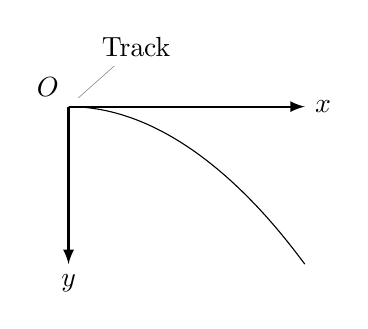
\begin{tikzpicture}
        %% NOTE: draw diagram
        %% labels and axis
        \node[anchor=south east] at (0,0) {$O$};
        \draw[thick,-latex] (0,0) -- (3,0) node[anchor=west] {$x$};
        \draw[thick,-latex] (0,0) -- (0,-2) node[anchor=north] {$y$};
        %% track
        \draw (0,0) parabola bend (0,0) (3,-2) node[pos=0.5,pin={60:Track}] {};
    \end{tikzpicture}
    \end{center}
    The $x$- and $y$-coordinates of the track are related in dimensionless units
        by $y=\frac{x^2}{4}$, where the positive $y$-axis is in the vertical downward direction.
    As the particle slides down the track,
        what is its tangential acceleration?
    \begin{multicols}{2}
    \begin{choices}
        \wrongchoice{zero}
        \wrongchoice{$g$}
        \wrongchoice{$\dfrac{gx}{2}$}
        \wrongchoice{$\dfrac{gx}{\sqrt{x^2+4}}$}
        \wrongchoice{$\dfrac{gx^2}{\sqrt{x^2+16}}$}
    \end{choices}
    \end{multicols}
\end{question}
}

\element{gre}{
\begin{question}{GRE8677-Q07}
    A \SI{2.0}{\kilo\gram} box hangs by a massless rope from a ceiling.
    A force slowly pulls the box horizontally to the side until the horizontal force is \SI{10}{\newton}.
    The box is then in equilibrium as shown below.
    \begin{center}
    %% NOTE: TODO: only templated
    \begin{tikzpicture}
        %% Ceiling
        \node[anchor=south,fill,pattern=north east lines,minimum width=4cm, minimum height=0.05cm] at (0,0) {};
        \draw (-2,0) -- (2,0);
        %% Pendulum Bob
        \node[fill,draw,circle,minimum size=1em] (A) at (225:3cm) {};
        \draw (0,0) -- (A);
        %% Circular path
        \draw[dashed] (0,-2.21) circle (2.21cm and 0.5cm);
        %% Angle
        \draw[dashed] (0,0) -- (0,-2.21);
        \draw[<->] (225:1cm) arc (225:270:1cm) node[pos=0.5,anchor=north] {$\theta$};
    \end{tikzpicture}
    \end{center}
    The angle that the rope makes with the vertical is closest to:
    \begin{multicols}{2}
    \begin{choices}
        \wrongchoice{$\mathrm{arctan}\,\num{0.5}$}
        \wrongchoice{$\mathrm{arcsin}\,\num{0.5}$}
        \wrongchoice{$\mathrm{arctan}\,\num{2.0}$}
        \wrongchoice{$\mathrm{arcsin}\,\num{2.0}$}
        \wrongchoice{\ang{45}}
    \end{choices}
    \end{multicols}
\end{question}
}

\element{gre}{
\begin{question}{GRE8677-Q08}
    A \SI{5.0}{\kilo\gram} stone is dropped on a nail and drives the nail \SI{0.025}{\meter} into a piece of wood.
    If the stone is moving at \SI{10}{\meter\per\second} when it hits the nail,
        the average force exerted on the nail by the stone while the nail is going into the wood is most nearly:
    \begin{multicols}{2}
    \begin{choices}
        \wrongchoice{\SI{10}{\newton}}
        \wrongchoice{\SI{100}{\newton}}
        \wrongchoice{\SI{1000}{\newton}}
        \wrongchoice{\SI{10000}{\newton}}
        \wrongchoice{\SI{100000}{\newton}}
    \end{choices}
    \end{multicols}
\end{question}
}

\element{gre}{
\begin{question}{GRE8677-Q09}
    A wire of diameter \SI{0.02}{\meter} contains \num{1e28} free electrons per cubic meter.
    For an electric current of \SI{100}{\ampere}, the drift velocity for free electrons in the wire is most nearly:
    \begin{multicols}{2}
    \begin{choices}
        \wrongchoice{\SI{0.6e-29}{\meter\per\second}}
        \wrongchoice{\SI{1e-19}{\meter\per\second}}
        \wrongchoice{\SI{5e-10}{\meter\per\second}}
        \wrongchoice{\SI{2e-4}{\meter\per\second}}
        \wrongchoice{\SI{8e3}{\meter\per\second}}
    \end{choices}
    \end{multicols}
\end{question}
}

\element{gre}{
\begin{question}{GRE8677-Q10}
    An isolated sphere of radius $R$ contains a uniform volume distribution of positive charge.
    \begin{center}
    \begin{tikzpicture}
        %% NOTE:
    \end{tikzpicture}
    \end{center}
    Which of the curves on the graph above correctly illustrates
        the dependence of the magnitude of the electric field of
        the sphere as a function of the distance $f$ from its center?
    \begin{multicols}{2}
    \begin{choices}
        \wrongchoice{\SI{0.6e-29}{\meter\per\second}}
        \wrongchoice{\SI{1e-19}{\meter\per\second}}
        \wrongchoice{\SI{5e-10}{\meter\per\second}}
        \wrongchoice{\SI{2e-4}{\meter\per\second}}
        \wrongchoice{\SI{8e3}{\meter\per\second}}
    \end{choices}
    \end{multicols}
\end{question}
}


%% Page 19
\element{gre}{
\begin{question}{GRE8677-Q11}
    Which of the following equations is a consequence of the equation
    \begin{displaymath}
        \nabla\times\mathbf{H} = \mathbf{\dot{D}} + \mathbf{J} ?
    \end{displaymath}
    \begin{multicols}{2}
    \begin{choices}
        \wrongchoice{$\nabla\cdot\left(\mathbf{\dot{D}} + \mathbf{J}\right)=0$}
        \wrongchoice{$\nabla\times\left(\mathbf{\dot{D}} + \mathbf{J}\right)=0$}
        \wrongchoice{$\nabla\left(\mathbf{\dot{D}}\cdot\mathbf{J}\right)=0$}
        \wrongchoice{$\mathbf{\dot{D}} + \mathbf{J}=0$}
        \wrongchoice{$\mathbf{\dot{D}}\cdot\mathbf{J}=0$}
    \end{choices}
    \end{multicols}
\end{question}
}

\element{gre}{
\begin{question}{GRE8677-Q12}
    A source of \SI{1}{\kilo\hertz} sound is moving straight toward you at a speed \num{0.9} times the speed of sound.
    The frequency you receive is:
    \begin{multicols}{2}
    \begin{choices}
        \wrongchoice{\SI{0.1}{\kilo\hertz}}
        \wrongchoice{\SI{0.5}{\kilo\hertz}}
        \wrongchoice{\SI{1.1}{\kilo\hertz}}
        \wrongchoice{\SI{1.9}{\kilo\hertz}}
        \wrongchoice{\SI{10}{\kilo\hertz}}
    \end{choices}
    \end{multicols}
\end{question}
}

\element{gre}{
\begin{question}{GRE8677-Q13}
    Two coherent sources of visible monochromatic light form an interference pattern on a screen.
    If the relative phase of the sources is varied from 0 to $2\pi$ at a frequency of \SI{500}{\hertz},
        which of the following best describes the effect,
        if any, on the interference pattern?
    \begin{choices}
        \wrongchoice{It is unaffected because the frequency of the phase change is very small compared to the frequency of visible light.}
        \wrongchoice{It is unaffected because the frequency of the phase change is an integral multiple of $\pi$.}
        \wrongchoice{It is destroyed except when the phase difference is 0 or $\pi$.}
        \wrongchoice{It is destroyed for all phase differences because the monochromaticity of the sources is destroyed.}
        \wrongchoice{It is not destroyed but shifts positions at a rate too rapid to be detected by the eye.}
    \end{choices}
\end{question}
}

\element{gre}{
\begin{question}{GRE8677-Q14}
    For an ideal gas, the specific heat at constant pressure $C_p$ is greater than the specific heat at constant volume $C_v$ because the:
    \begin{choices}
        \wrongchoice{gas does work on its environment when its pressure remains constant while its temperature is increased}
        \wrongchoice{heat input per degree increase in temperature is the same in processes for which either the pressure or the volume is kept constant.}
        \wrongchoice{pressure of the gas remains constant when its temperature remains constant.}
        \wrongchoice{increase in the gas's internal energy is greater when the pressure remains constant than when the volume remains constant.}
        \wrongchoice{heat needed is greater when the volume remains constant than when the pressure remains constant.}
    \end{choices}
\end{question}
}

\element{gre}{
\begin{question}{GRE8677-Q15}
    A sample of $N$ atoms of helium gas is confined in a 1.0 cubic meter volume.
    The probability that none of the helium atoms is in a \num{1.0e-6} cubic meter volume of the container is:
    \begin{multicols}{2}
    \begin{choices}
        \wrongchoice{zero}
        \wrongchoice{$\left(10^{-6}\right)^{N}$}
        \wrongchoice{$\left(1-10^{-6}\right)^{N}$}
        \wrongchoice{$1-\left(10^{-6}\right)^{N}$}
        \wrongchoice{one}
    \end{choices}
    \end{multicols}
\end{question}
}

\element{gre}{
\begin{question}{GRE8677-Q16}
    Except for mass, the properties of the muon most closely resemble the properties of the:
    \begin{multicols}{2}
    \begin{choices}
        \wrongchoice{electron}
        \wrongchoice{graviton}
        \wrongchoice{photon}
        \wrongchoice{pion}
        \wrongchoice{proton}
    \end{choices}
    \end{multicols}
\end{question}
}

%% Page 20

\element{gre}{
\begin{question}{GRE8677-Q17}
    Suppose that \ce{^{A}_{Z}X} decays by natural radioactivity in two stages to \ce{^{A-4}_{Z-1}Y}.
    The two stages would most likely be which of the following?
    \begin{multicols}{2}
    \begin{choices}
        %% NOTE: table options
        \wrongchoice{proton}
    \end{choices}
    \end{multicols}
\end{question}
}

\element{gre}{
\begin{question}{GRE8677-Q18}
    The wave function $\Psi(x) = A \mathrm{exp}\left(-\dfrac{b^2x^2}{2}\right)$,
        where $A$ and $b$ are real constants,
        is normalized eigenfunction of the Schr\"{o}dinger equation for a particle of mass $M$ and energy $E$ in a one dimensional potential $V(x)$ such that $V(x)=0$ at $x=0$.
    Which of the following is correct?
    \begin{multicols}{2}
    \begin{choices}
        \wrongchoice{$V = \dfrac{\hbar^2 b^4}{2M}$}
        \wrongchoice{$V = \dfrac{\hbar^2 b^4 x^2}{2M}$}
        \wrongchoice{$V = \dfrac{\hbar^2 b^8 x^4}{2M}$}
        \wrongchoice{$E = \hbar^2 b^2 \left(1-b^2 x^2\right)$}
        \wrongchoice{$E = \dfrac{\hbar^2 b^2}{2M}$}
    \end{choices}
    \end{multicols}
\end{question}
}

\element{gre}{
\begin{question}{GRE8677-Q19}
    The energy levels of the hydrogen atom are given in terms of the principle quantum number $n$ and a positive constant $A$ by the expression:
    \begin{multicols}{2}
    \begin{choices}
        \wrongchoice{$A \left(n+\dfrac{1}{2}\right)$}
        \wrongchoice{$A \left(1-n^2\right)$}
        \wrongchoice{$A \left(-\dfrac{1}{4}+\dfrac{1}{n^2}\right)$}
        \wrongchoice{$A n^2$}
        \wrongchoice{$-\dfrac{A}{n^2}$}
    \end{choices}
    \end{multicols}
\end{question}
}

\element{gre}{
\begin{question}{GRE8677-Q20}
    A positive kaon $(K^+)$ has a rest mass of \SI{494}{\mega\eV\per\clight\squared}.
    If a kaon has a total energy that is equal to the proton rest energy,
        the speed of the kaon is most nearly:
    \begin{multicols}{2}
    \begin{choices}
        \wrongchoice{\SI{0.25}{\clight}}
        \wrongchoice{\SI{0.40}{\clight}}
        \wrongchoice{\SI{0.55}{\clight}}
        \wrongchoice{\SI{0.70}{\clight}}
        \wrongchoice{\SI{0.85}{\clight}}
    \end{choices}
    \end{multicols}
\end{question}
}

\element{gre}{
\begin{question}{GRE8677-Q21}
    Two observers $O$ and $O^{\prime}$ observe two events $A$ and $B$.
    The observers have a constant relative speed of \SI{0.8}{\clight}.
    In units such that the speed of light is one, observer $O$ obtained the following coordinates:
    \begin{description}
        \item[Event $A$:] $x=3$, $y=3$, $z=3$, $t=3$
        \item[Event $B$:] $x=5$, $y=3$, $z=1$, $t=5$
    \end{description}
    What is the length of the space-time interval between these two events,
        as measured by $O^{\prime}$?
    \begin{multicols}{3}
    \begin{choices}
        \wrongchoice{$1$}
        \wrongchoice{$\sqrt{2}$}
        \wrongchoice{$2$}
        \wrongchoice{$3$}
        \wrongchoice{$2\sqrt{3}$}
    \end{choices}
    \end{multicols}
\end{question}
}

\element{gre}{
\begin{question}{GRE8677-Q22}
    Which of the following statements most accurately describes how an electromagnetic field behaves under a Lorentz transformation?
    \begin{choices}
        \wrongchoice{The electric field transformed completely into a magnetic field.}
        \wrongchoice{If initially there is only an electric field, after the transformation there may be both an electric and a magnetic field.}
        \wrongchoice{The electric field is unaltered.}
        \wrongchoice{The magnetic field is unaltered.}
        \wrongchoice{It cannot be determined unless gauge transformation is also specified.}
    \end{choices}
\end{question}
}

\element{gre}{
\begin{question}{GRE8677-Q23}
    Which of the following statements concerning the electrical conductivities at room temperature of a pure copper sample and a pure silicon sample is \emph{not} true?
    \begin{choices}
        \wrongchoice{The conductivity of the copper sample is many orders of magnitude greater than that of the silicon sample.}
        \wrongchoice{If the temperature of the copper sample is increased, its conductivity will decrease.}
        \wrongchoice{If the temperature of the silicon sample is increased, its conductivity will increase.}
        \wrongchoice{The addition of an impurity in the copper sample always decreases its conductivity.}
        \wrongchoice{The addition of an impurity in the silicon sample always decreases its conductivity.}
    \end{choices}
\end{question}
}

%% Page 21

\element{gre}{
\begin{question}{GRE8677-Q24}
    The batter in the diagram above is to be charged by the generator $G$.
    The generator has a terminal voltage of 120 volts when the charging current is 10 amperes.
    The batter has an emf of 100 volts and an internal resistance of 1 ohm.
    \begin{center}
    \begin{tikzpicture}
        %% NOTE:
    \end{tikzpicture}
    \end{center}
    In order to charge the battery at 100 amperes charging current,
        the resistance $R$ should be set at:
    \begin{multicols}{3}
    \begin{choices}
        \wrongchoice{\SI{0.1}{\ohm}}
        \wrongchoice{\SI{0.5}{\ohm}}
        \wrongchoice{\SI{1.0}{\ohm}}
        \wrongchoice{\SI{5.0}{\ohm}}
        \wrongchoice{\SI{10.0}{\ohm}}
    \end{choices}
    \end{multicols}
\end{question}
}

\element{gre}{
\begin{question}{GRE8677-Q25}
    A charged particle is released from rest in a region where there is a constant electric field and a constant magnetic field.
    If the two fields are parallel to each other,
        the path of the particle is a:
    \begin{multicols}{2}
    \begin{choices}
        \wrongchoice{circle}
        \wrongchoice{parabola}
        \wrongchoice{helix}
        \wrongchoice{cycloid}
        \wrongchoice{straight line}
    \end{choices}
    \end{multicols}
\end{question}
}

\element{gre}{
\begin{question}{GRE8677-Q26}
    A nickel target ($Z=28$) is bombarded with fast electrons.
    The minimum electron kinetic energy needed to produce x-rays in the $K$ series is most nearly:
    \begin{multicols}{2}
    \begin{choices}
        \wrongchoice{\SI{10}{\eV}}
        \wrongchoice{\SI{100}{\eV}}
        \wrongchoice{\SI{1000}{\eV}}
        \wrongchoice{\SI{10 000}{\eV}}
        \wrongchoice{\SI{100 000}{\eV}}
    \end{choices}
    \end{multicols}
\end{question}
}

\element{gre}{
\begin{question}{GRE8677-Q27}
    The hypothesis that an electron possesses spin is qualitatively significant for the explanation of all of the following topics \emph{except} the:
    \begin{choices}
        \wrongchoice{structure of the periodic table}
        \wrongchoice{specific heat of metals}
        \wrongchoice{anomalous Zeeman effect}
        \wrongchoice{deflection of a moving electron by a uniform magnetic field}
        \wrongchoice{fine structure of atomic spectra}
    \end{choices}
\end{question}
}

\element{gre}{
\begin{question}{GRE8677-Q28}
    Eigenfunctions for a rigid dumbbell rotating about its center have a $\phi$ dependence of the form $\Psi(\phi) = A\mathrm{e}^{im\phi}$,
        where $m$ is a quantum number and $A$ is a constant.
    Which of the following values of $A$ will properly normalize the eigenfunction?
    \begin{multicols}{3}
    \begin{choices}
        \wrongchoice{$\sqrt{2\pi}$}
        \wrongchoice{$2\pi$}
        \wrongchoice{$\left(2\pi\right)^2$}
        \wrongchoice{$\dfrac{1}{\sqrt{2\pi}}$}
        \wrongchoice{$\dfrac{1}{2\pi}$}
    \end{choices}
    \end{multicols}
\end{question}
}

\element{gre}{
\begin{question}{GRE8677-Q29}
    A negative test charge is moving near a long straight wire in which there is a current.
    A force will act on the test charge in a direction parallel to the direction of the current if the motion of the charge is in a direction:
    \begin{choices}
        \wrongchoice{toward the wire}
        \wrongchoice{away from the wire}
        \wrongchoice{the same as that of the current}
        \wrongchoice{opposite to that of the current}
        \wrongchoice{perpendicular to both the direction of the current and the direction toward the wire}
    \end{choices}
\end{question}
}

\element{gre}{
\begin{question}{GRE8677-Q30}
    The configuration of the potassium atom in its ground state is $1s^2$ $2s^2$ $2p^6$ $3s^2$ $3p^6$ $4s^1$.
    Which of the following statements about potassium is true?
    \begin{choices}
        \wrongchoice{Its $n=3$ shell is completely filled.}
        \wrongchoice{Its $4s$ subshell is completely filled.}
        \wrongchoice{Its least tightly bound electron has $l=4$}
        \wrongchoice{Its atomic number is 17}
        \wrongchoice{Its electron charge distribution is spherically symmetrical.}
    \end{choices}
\end{question}
}

%% Page 22

\element{gre}{
\begin{question}{GRE8677-Q31}
    In this apparatus, the photocathode and the collector are made from the same material.
    \begin{center}
    \begin{tikzpicture}
        %% NOTE:
    \end{tikzpicture}
    \end{center}
    The potential $V$ of the collector, measured relative to ground, is initially zero and is then increased or decreased monotonically.
    The effect is described by Einstein's photoelectric equation.
    \begin{equation*}
        |eV| = h\nu - W.
    \end{equation*}
    %% Begin question
    When the photoelectric equation is satisfied and applicable to this situation,
        $V$ is the:
    \begin{choices}
        \wrongchoice{negative value at which the current stops}
        \wrongchoice{negative value at which the current starts}
        \wrongchoice{positive value at which the current stops}
        \wrongchoice{positive value at which the current starts}
        \wrongchoice{voltage induced when the light is on}
    \end{choices}
\end{question}
}

\element{gre}{
\begin{question}{GRE8677-Q32}
    In this apparatus, the photocathode and the collector are made from the same material.
    \begin{center}
    \begin{tikzpicture}
        %% NOTE:
    \end{tikzpicture}
    \end{center}
    The potential $V$ of the collector, measured relative to ground, is initially zero and is then increased or decreased monotonically.
    The effect is described by Einstein's photoelectric equation.
    \begin{equation*}
        |eV| = h\nu - W.
    \end{equation*}
    %% Begin question
    The photoelectric equation is derived under the assumption that:
    \begin{choices}
        \wrongchoice{electrons are restricted to orbits of angular momentum $n\hbar$, where $n$ is an integer}
        \wrongchoice{electrons are associated with waves of wavelength $\lambda=h/p$, where $p$ is momentum}
        \wrongchoice{light is emitted only when electrons jump between orbits}
        \wrongchoice{light is absorbed in quanta of energy $E=h\nu$}
        \wrongchoice{light behaves like a wave}
    \end{choices}
\end{question}
}

\element{gre}{
\begin{question}{GRE8677-Q33}
    In this apparatus, the photocathode and the collector are made from the same material.
    \begin{center}
    \begin{tikzpicture}
        %% NOTE:
    \end{tikzpicture}
    \end{center}
    The potential $V$ of the collector, measured relative to ground, is initially zero and is then increased or decreased monotonically.
    The effect is described by Einstein's photoelectric equation.
    \begin{equation*}
        |eV| = h\nu - W.
    \end{equation*}
    %% Begin question
    The quantity $W$ in the photoelectric equation is the:
    \begin{choices}
        \wrongchoice{energy difference between the two lowest electron orbits in the atoms of the photocathode}
        \wrongchoice{total light energy absorbed by the photocathode during the measurement}
        \wrongchoice{minimum energy a photon must have in order to be absorbed by the photocathode}
        \wrongchoice{minimum energy required to free an electron from its binding to the cathode material}
        \wrongchoice{average energy of all electrons in the photocathode}
    \end{choices}
\end{question}
}

%% Page 23


\element{gre}{
\begin{question}{GRE8677-Q34}
    The potential energy of a body constrained to move on a straight line is $kx^4$
        where $K$ is a constant.
    The position of the body is $x$, its speed $v$, its linear momentum $p$,
        and its mass $m$.
    %% Start Question
    The force on the body is:
    \begin{multicols}{3}
    \begin{choices}
        \wrongchoice{$\dfrac{1}{2}mv^2$}
        \wrongchoice{$-4kx^3$}
        \wrongchoice{$4kx^4$}
        \wrongchoice{$-\dfrac{4kx^5}{5}$}
        \wrongchoice{$mg$}
    \end{choices}
    \end{multicols}
\end{question}
}

\element{gre}{
\begin{question}{GRE8677-Q35}
    The potential energy of a body constrained to move on a straight line is $kx^4$
        where $K$ is a constant.
    The position of the body is $x$, its speed $v$, its linear momentum $p$,
        and its mass $m$.
    %% Start Question
    The hamiltonian for this system is:
    \begin{multicols}{2}
    \begin{choices}
        \wrongchoice{$\dfrac{p^2}{2m} + kx^4$}
        \wrongchoice{$\dfrac{p^2}{2m} - kx^4$}
        \wrongchoice{$kx^4$}
        \wrongchoice{$\dfrac{1}{2}mv^2 - kx^4$}
        \wrongchoice{$\dfrac{1}{2}mv^2$}
    \end{choices}
    \end{multicols}
\end{question}
}

\element{gre}{
\begin{question}{GRE8677-Q36}
    The potential energy of a body constrained to move on a straight line is $kx^4$
        where $K$ is a constant.
    The position of the body is $x$, its speed $v$, its linear momentum $p$,
        and its mass $m$.
    %% Start Question
    The body moves from $x_1$ at time $t_1$ to $x_2$ at time $t_2$.
    Which of the following quantities is an extremum for the $x-t$ curve corresponding to this motion,
        if end points are fixed?
    \begin{multicols}{2}
    \begin{choices}
        \wrongchoice{$\int^{t_2}_{t_1}\,\left(\dfrac{1}{2}mv^2 - kx^4\right)\,\mathrm{d}t$}
        \wrongchoice{$\int^{t_2}_{t_1}\,\left(\dfrac{1}{2}mv^2\right)\,\mathrm{d}t$}
        \wrongchoice{$\int^{t_2}_{t_1}\,\left(mxv\right)\,\mathrm{d}t$}
        \wrongchoice{$\int^{t_2}_{t_1}\,\left(\dfrac{1}{2}mv^2 + kx^4\right)\,\mathrm{d}x$}
        \wrongchoice{$\int^{t_2}_{t_1}\,\left(mv\right)\,\mathrm{d}x$}
    \end{choices}
    \end{multicols}
\end{question}
}

%% GRE-A8
\element{gre}{
\begin{question}{GRE8677-Q37}
    %% NOTE: tikz
    The figure above represents a point mass $m$ attached to the ceiling by a cord of fixed length $l$.
    If the point mass moves in a horizontal circle of radius $r$ with uniform angular velocity $\omega$,
        the tension in the cord is:
    \begin{multicols}{2}
    \begin{choices}
        \wrongchoice{$mg\left(\dfrac{r}{l}\right)$}
        \wrongchoice{$mg\cos\left(\dfrac{\theta}{2}\right)$}
        \wrongchoice{$\dfrac{m\omega r}{\sin\left(\dfrac{\theta}{2}\right)}$}
        \wrongchoice{$m\sqrt{\omega^2 r^2 + g^2}$}
        \wrongchoice{$m\sqrt{\omega^4 r^2 + g^2}$}
    \end{choices}
    \end{multicols}
\end{question}
}

\element{gre}{
\begin{question}{GRE8677-Q38}
    %% NOTE: tikz
    If logical $O$ is 0 volts and logical 1 is $+1$ volt,
        the circuit shown above is a logic circuit commonly known as
    \begin{multicols}{2}
    \begin{choices}
        \wrongchoice{an OR gate}
        \wrongchoice{an AND gate}
        \wrongchoice{a 2 bit adder}
        \wrongchoice{a flip flop}
        \wrongchoice{a fanout}
    \end{choices}
    \end{multicols}
\end{question}
}

%% Page 24

\element{gre}{
\begin{question}{GRE8677-Q39}
    %% NOTE: big tikz
    The gain of an amplifier is plotted \emph{verses} angular frequency $\omega$ in the diagram above.
    If $K$ and $a$ are positive constants, the frequency dependence of the gain near $\omega=\num{3e5}$ seconds$^{-1}$ is most accurately expressed by:
    \begin{multicols}{3}
    \begin{choices}
        \wrongchoice{$K\mathrm{e}^{-a\omega}$}
        \wrongchoice{$K\omega^2$}
        \wrongchoice{$K\omega$}
        \wrongchoice{$K\omega^{-1}$}
        \wrongchoice{$K\omega^{-2}$}
    \end{choices}
    \end{multicols}
\end{question}
}

%% Page 25

\element{gre}{
\begin{question}{GRE8677-Q40}
    An experimenter measured 9934 counts during one hour from a radioactive sample.
    From this number the counting rate of the sample can be estimated with a standard deviation of most nearly:
    \begin{multicols}{3}
    \begin{choices}
        \wrongchoice{100}
        \wrongchoice{200}
        \wrongchoice{300}
        \wrongchoice{400}
        \wrongchoice{500}
    \end{choices}
    \end{multicols}
\end{question}
}

\element{gre}{
\begin{question}{GRE8677-Q41}
    Which of the following nuclei has the largest binding energy per nucleon?
    (consider the most abundant isotope of each element.)
    \begin{multicols}{2}
    \begin{choices}
        \wrongchoice{Helium}
        \wrongchoice{Carbon}
        \wrongchoice{Iron}
        \wrongchoice{Uranium}
        \wrongchoice{Plutonium}
    \end{choices}
    \end{multicols}
\end{question}
}

\element{gre}{
\begin{question}{GRE8677-Q42}
    A proton beam is incident on a scatterer 0.1 centimeter thick.
    The scatterer contains \num{e20} target nuclei per cubic centimeter.
    In passing through the scatterer,
        one proton per incident million is scattered.
    The scattering cross section is:
    \begin{multicols}{2}
    \begin{choices}
        \wrongchoice{\SI{e-29}{\centi\meter\squared}}
        \wrongchoice{\SI{e-27}{\centi\meter\squared}}
        \wrongchoice{\SI{e-25}{\centi\meter\squared}}
        \wrongchoice{\SI{e-23}{\centi\meter\squared}}
        \wrongchoice{\SI{e-21}{\centi\meter\squared}}
    \end{choices}
    \end{multicols}
\end{question}
}

\element{gre}{
\begin{question}{GRE8677-Q43}
    %% NOTE: tikz
    Three masses are connected by two springs as shown above.
    A longitudinal normal mode with frequency $\dfrac{1}{2\pi}\sqrt{\dfrac{k}{m}}$ is exhibited by:
    \begin{choices}
        \wrongchoice{$A$, $B$, $C$ all moving in the same direction with equal amplitude}
        \wrongchoice{$A$ and $C$ moving in opposite directions with equal amplitude}
        \wrongchoice{$A$ and $C$ moving in the same direction with equal amplitude, and $B$ moving in the opposite direction with the same amplitude}
        \wrongchoice{$A$ and $C$ moving in the same direction with equal amplitude, and $B$ moving in the opposite direction with twice the amplitude}
        \wrongchoice{none of the provided}
    \end{choices}
\end{question}
}

\element{gre}{
\begin{question}{GRE8677-Q44}
    %% NOTE: tikz
    A uniform stick of length $L$ and mass $M$ lies on a frictionless horizontal surface.
    A point particle of mass $m$ approached the stick with speed $v$ on a straight line perpendicular to the stick that intersects the stick at one end,
        as shown above.
    After the collision,
        which is elastic, the particle is at rest.
    The speed $V$ of the center of mass of the stick after the collision is:
    \begin{multicols}{2}
    \begin{choices}
        \wrongchoice{$\dfrac{m}{M}v$}
        \wrongchoice{$\dfrac{m}{M+m}v$}
        \wrongchoice{$\sqrt{\dfrac{m}{M}}v$}
        \wrongchoice{$\sqrt{\dfrac{m}{M+m}}v$}
        \wrongchoice{$\dfrac{3m}{M}v$}
    \end{choices}
    \end{multicols}
\end{question}
}

\element{gre}{
\begin{question}{GRE8677-Q45}
    Photons of wavelength $\lambda$ scatter elastically on free protons initially at rest.
    The wavelength of the photons scattered at \ang{90} is increased by:
    \begin{choices}
        \wrongchoice{$\dfrac{\lambda}{137}$}
        \wrongchoice{$\dfrac{\lambda}{1836}$}
        \wrongchoice{$\dfrac{\lambda}{m_e c}$, where $h$ is Planck's constant, $m_e$ the rest mass of an electron, and $c$ the speed of light.}
        \wrongchoice{$\dfrac{\lambda}{m_p c}$, where $h$ is Planck's constant, $m_p$ the rest mass of a proton, and $c$ the speed of light.}
        \wrongchoice{zero}
    \end{choices}
\end{question}
}

%% Page 26

\element{gre}{
\begin{question}{GRE8677-Q46}
    A blackbody at temperature $T_1$ radiates energy at a power level of 10 milliwatts (\si{\milli\watt}).
    The same blackbody, when at temperature $2T_1$, radiates energy at a power level of:
    \begin{multicols}{2}
    \begin{choices}
        \wrongchoice{\SI{10}{\milli\watt}}
        \wrongchoice{\SI{20}{\milli\watt}}
        \wrongchoice{\SI{40}{\milli\watt}}
        \wrongchoice{\SI{80}{\milli\watt}}
        \wrongchoice{\SI{160}{\milli\watt}}
    \end{choices}
    \end{multicols}
\end{question}
}

\element{gre}{
\begin{question}{GRE8677-Q47}
    The Frank-Hertz experiment and related scattering experiments show that:
    \begin{choices}
        \wrongchoice{electrons are always scattered elastically from atoms}
        \wrongchoice{electrons are never scattered elastically from atoms}
        \wrongchoice{electrons of a certain energy range can be scattered inelastically, and the energy lost by electrons is discrete}
        \wrongchoice{electrons always lost the same energy when they are scattered inelastically}
        \wrongchoice{there is no energy range in which the energy lost by electrons varies continuously}
    \end{choices}
\end{question}
}

\element{gre}{
\begin{question}{GRE8677-Q48}
    A transition in which one photon is radiated by the electron in a hydrogen atom when the electron's wave function changes from $\Phi_1$ to $\Phi_2$ is forbidden if $\Phi_1$ and $\Phi_2$:
    \begin{choices}
        \wrongchoice{have opposite parity}
        \wrongchoice{are orthogonal to each other}
        \wrongchoice{are zero at the center of the atomic nucleus}
        \wrongchoice{are both spherically symmetrical}
        \wrongchoice{are associated with different angular momenta}
    \end{choices}
\end{question}
}

\element{gre}{
\begin{question}{GRE8677-Q49}
    The Hamiltonian operator in the Schr\"{o}dinger equation can be formed from the classical Hamiltonian by substituting:
    \begin{choices}
        \wrongchoice{wavelength and frequency for momentum and energy}
        \wrongchoice{a differential operator for momentum}
        \wrongchoice{transition probability for potential energy}
        \wrongchoice{sums over discrete eigenvalues for integrals over continuous variables}
        \wrongchoice{Gaussian distribution of observables for exact values}
    \end{choices}
\end{question}
}

\element{gre}{
\begin{question}{GRE8677-Q50}
    The Hall effect is used in solid-state physics to measure:
    \begin{choices}
        \wrongchoice{ratio of charge to mass}
        \wrongchoice{magnetic susceptibility}
        \wrongchoice{the sign of the charge carriers}
        \wrongchoice{the width of the gap between the conduction and valence bands}
        \wrongchoice{Fermi energy}
    \end{choices}
\end{question}
}

\element{gre}{
\begin{question}{GRE8677-Q51}
    One feature common to both the Debye theory and the Einstein theory of the specific heat of a crystal composed of $N$ identical atoms is that the:
    \begin{choices}
        \wrongchoice{average energy of each atom is $3kt$}
        \wrongchoice{vibrational energy of the crystal is equivalent to the energy of $3N$ independent harmonic oscillators}
        \wrongchoice{crystal is assumed to be continuous for all elastic waves}
        \wrongchoice{speed of the longitudinal elastic waves is less than the speed of the transverse elastic waves}
        \wrongchoice{upper cutoff frequency of the elastic waves is the same}
    \end{choices}
\end{question}
}

\element{gre}{
\begin{question}{GRE8677-Q52}
    A cube has a constant electric potential $V$ on its surface.
    If there are no charges inside the cube,
        the potential at the center of the cube is:
    \begin{multicols}{3}
    \begin{choices}
        \wrongchoice{zero}
        \wrongchoice{$\dfrac{V}{8}$}
        \wrongchoice{$\dfrac{V}{6}$}
        \wrongchoice{$\dfrac{V}{2}$}
        \wrongchoice{$V$}
    \end{choices}
    \end{multicols}
\end{question}
}

\element{gre}{
\begin{question}{GRE8677-Q53}
    A charged particle oscillates harmonically along the $x$-axis as shown below.
    \begin{center}
    \begin{tikzpicture}
        %% NOTE:
    \end{tikzpicture}
    \end{center}
    The radiation from the particle is detected at a distant point $P$,
        which lies in the $xy$-plane.
    The electric field at $P$ is in the:
    \begin{choices}
        \wrongchoice{$\pm z$ direction and has a maximum amplitude at $\theta=\ang{90}$}
        \wrongchoice{$\pm z$ direction and has a minimum amplitude at $\theta=\ang{90}$}
        \wrongchoice{$xy$-plane and has a maximum amplitude at $\theta=\ang{90}$}
        \wrongchoice{$xy$-plane and has a minimum amplitude at $\theta=\ang{90}$}
        \wrongchoice{$xy$-plane and has a maximum amplitude at $\theta=\ang{45}$}
    \end{choices}
\end{question}
}

%% Page 27

\element{gre}{
\begin{question}{GRE8677-Q54}
    A dielectric of dielectric constant $K$ is placed in contact with a conductor having surface charge density $\sigma$,
        as shown below.
    \begin{center}
    \begin{tikzpicture}
        %% NOTE:
    \end{tikzpicture}
    \end{center}
    What is the polarization (bound) charge density $\sigma_p$ on the surface of the dielectric at the interface between the two materials?
    \begin{multicols}{3}
    \begin{choices}
        \wrongchoice{$\sigma\dfrac{K}{1-K}$}
        \wrongchoice{$\sigma\dfrac{K}{1+K}$}
        \wrongchoice{$\sigma K$}
        \wrongchoice{$\sigma\dfrac{1+K}{K}$}
        \wrongchoice{$\sigma\dfrac{1-K}{K}$}
    \end{choices}
    \end{multicols}
\end{question}
}

\element{gre}{
\begin{question}{GRE8677-Q55}
    The mean kinetic energy of electrons in metals at room temperature is usually many times the thermal energy $kT$.
    Which of the following can best be used to explain this fact?
    \begin{choices}
        \wrongchoice{The energy-time uncertainty relation}
        \wrongchoice{The Pauli-exclusion principle}
        \wrongchoice{The degeneracy of the energy levels}
        \wrongchoice{The Born approximation}
        \wrongchoice{The wave-particle duality}
    \end{choices}
\end{question}
}

\element{gre}{
\begin{question}{GRE8677-Q56}
    If $\Psi$ is a normalized solution of the Schr\"{o}dinger equation and $Q$ is the operator corresponding to a physical observable $x$,
        the quantity $\Psi^{\ast}Q\Psi$ may be integrated in order to obtain the:
    \begin{choices}
        \wrongchoice{normalized constant for $\Psi$}
        \wrongchoice{spatial overlap of $Q$ with $\Psi$}
        \wrongchoice{mean value of $x$}
        \wrongchoice{uncertainty in $x$}
        \wrongchoice{time derivative of $x$}
    \end{choices}
\end{question}
}

\element{gre}{
\begin{question}{GRE8677-Q57}
    Which of the following is an eigenfunction of the linear momentum operator $-i\hbar \dfrac{\partial}{\partial x}$ with a positive eigenvalue $\hbar k$,
        i.e., an eigenfunction that describes a particle that is moving in free space in the direction of positive $x$ with a precise value of linear momentum?
    \begin{multicols}{3}
    \begin{choices}
        \wrongchoice{$\cos kx$}
        \wrongchoice{$\sin kx$}
        \wrongchoice{$\mathrm{e}^{-i\hbar x}$}
        \wrongchoice{$\mathrm{e}^{i\hbar x}$}
        \wrongchoice{$\mathrm{e}^{-kx}$}
    \end{choices}
    \end{multicols}
\end{question}
}

\element{gre}{
\begin{question}{GRE8677-Q58}
    In an ordinary hologram, coherent monochromatic light produces a 3-dimensional picture because wave information is recorded for which of the following?
    \begin{itemize}
        \item[I.] Amplitude
        \item[II.] Phase
        \item[III.] Wave-front angular frequency
    \end{itemize}
    \begin{multicols}{2}
    \begin{choices}
        \wrongchoice{I only}
        \wrongchoice{I and II only}
        \wrongchoice{I and III only}
        \wrongchoice{II and III  only}
        \wrongchoice{I, II and III}
    \end{choices}
    \end{multicols}
\end{question}
}

\element{gre}{
\begin{question}{GRE8677-Q59}
    The dispersion law for a certain type of wave motion is $\omega=\left(c^2k^2+m^2\right)^{1/2}$,
        where $\omega$ is the angular frequency, $k$ is the magnitude of the propagation vector,
        and $c$ and $m$ are constants.
    The ground velocity of these waves approaches:
    \begin{choices}
        \wrongchoice{infinity as $k\to 0$ and zero as $k\to\infty$}
        \wrongchoice{infinity as $k\to 0$ and $c$ as $k\to\infty$}
        \wrongchoice{$c$ as $k\to 0$ and zero as $k\to\infty$}
        \wrongchoice{zero as $k\to 0$ and infinity as $k\to\infty$}
        \wrongchoice{zero as $k\to 0$ and $c$ as $k\to\infty$}
    \end{choices}
\end{question}
}

\element{gre}{
\begin{question}{GRE8677-Q60}
    A particle of mass $m$ that moves along the $x$-axis has potential energy $V(x) = x+bx^2$,
        where $a$ and $b$ are positive constants.
    Its initial velocity is $v_0$ at $x=0$.
    It will execute simple harmonic motion with a frequency determined by the value of:
    \begin{choices}
        \wrongchoice{$b$ alone}
        \wrongchoice{$b$ and $a$ alone}
        \wrongchoice{$b$ and $m$  alone}
        \wrongchoice{$b$, $a$, and $m$ alone}
        \wrongchoice{$b$, $a$, $m$ and $v_0$}
    \end{choices}
\end{question}
}


%% Page 28


\element{gre}{
\begin{question}{GRE8677-Q61}
    The equation of motion of a rocket in free space can be written
    \begin{equation*}
        m \dfrac{\mathrm{d}y}{\mathrm{d}t} + u \dfrac{\mathrm{d}m}{\mathrm{d}t} = 0
    \end{equation*}
    where $m$ is the rocket's mass, $v$ is its velocity, $t$ is time, and $u$ is a constant.
    %% Begin question
    The constant $u$ represents the speed of the:
    \begin{choices}
        \wrongchoice{rocket at $t=0$}
        \wrongchoice{rocket after its fuel is spent}
        \wrongchoice{rocket in its instantaneous rest frame}
        \wrongchoice{rocket's exhaust in a stationary frame}
        \wrongchoice{rocket's exhaust relative to the rocket}
    \end{choices}
\end{question}
}

\element{gre}{
\begin{question}{GRE8677-Q62}
    The equation of motion of a rocket in free space can be written
    \begin{equation*}
        m \dfrac{\mathrm{d}y}{\mathrm{d}t} + u \dfrac{\mathrm{d}m}{\mathrm{d}t} = 0
    \end{equation*}
    where $m$ is the rocket's mass, $v$ is its velocity, $t$ is time, and $u$ is a constant.
    %% Begin question
    The equation can be solved to give $v$ as a function of $m$.
    If the rocket has $m=m_0$ and $v=0$ when it starts,
        what is the solution?
    \begin{multicols}{2}
    \begin{choices}[o]
        \wrongchoice{$u \dfrac{m_0}{m}$}
        \wrongchoice{$u\,\mathrm{exp}\left(\dfrac{m_0}{m}\right)$}
        \wrongchoice{$u \sin\left(\dfrac{m_0}{m}\right)$}
        \wrongchoice{$u \tan\left(\dfrac{m_0}{m}\right)$}
        \wrongchoice{None of the above}
    \end{choices}
    \end{multicols}
\end{question}
}

\element{gre}{
\begin{question}{GRE8677-Q63}
    A point charge $-q$ coulombs is placed at a distance $d$ from a large grounded conducting plane.
    The surface charge density on the plane a distance $D$ from the point charge is:
    \begin{multicols}{3}
    \begin{choices}
        \wrongchoice{$\dfrac{q}{4\pi D}$}
        \wrongchoice{$\dfrac{q D^2}{2\pi}$}
        \wrongchoice{$\dfrac{q d}{2\pi D^2}$}
        \wrongchoice{$\dfrac{q d}{2\pi D^3}$}
        \wrongchoice{$\dfrac{q d}{4\pi\epsilon_0 D^2}$}
    \end{choices}
    \end{multicols}
\end{question}
}

\element{gre}{
\begin{question}{GRE8677-Q64}
    An alternating current electrical generator has a fixed internal impedance $R_g + jX_g$ and is used to supply power to a passive load that has an impedance $R_g + jX_l$,
        where $j=\sqrt{-1}$, $R_g\neq 0$, and $G_g \neq 0$.
    For maximum power transfer between the generator and the load,
        $X_l$ should be equal to:
    \begin{multicols}{3}
    \begin{choices}
        \wrongchoice{zero}
        \wrongchoice{$X_g$}
        \wrongchoice{$-X_g$}
        \wrongchoice{$R_g$}
        \wrongchoice{$-R_g$}
    \end{choices}
    \end{multicols}
\end{question}
}

\element{gre}{
\begin{question}{GRE8677-Q65}
    A current $i$ in a circular loop of radius $b$ produces a magnetic field.
    At a fixed point far from the loop, the strength of the magnetic field is proportional to which of the following combinations of $i$ and $b$?
    \begin{multicols}{3}
    \begin{choices}
        \wrongchoice{$ib$}
        \wrongchoice{$ib^2$}
        \wrongchoice{$i^2b$}
        \wrongchoice{$\dfrac{i}{b}$} %% ??
        \wrongchoice{$\dfrac{i}{b^2}$}
    \end{choices}
    \end{multicols}
\end{question}
}

\element{gre}{
\begin{question}{GRE8677-Q66}
    For a system in which the number of particles is fixed,
        the reciprocal of the Kelvin temperature $T$ is given by which of the following derivatives?
    (Let $P$=pressure, $V$=volume, $S$=entropy and $U$= internal energy.)
    \begin{multicols}{3}
    \begin{choices}
        \wrongchoice{$\left(\dfrac{\partial P}{\partial V}\right)_S$}
        \wrongchoice{$\left(\dfrac{\partial P}{\partial S}\right)_V$}
        \wrongchoice{$\left(\dfrac{\partial S}{\partial P}\right)_U$}
        \wrongchoice{$\left(\dfrac{\partial V}{\partial P}\right)_U$}
        \wrongchoice{$\left(\dfrac{\partial S}{\partial U}\right)_V$}
    \end{choices}
    \end{multicols}
\end{question}
}

\element{gre}{
\begin{question}{GRE8677-Q67}
    A large isolated system of $N$ weakly interacting particles is in thermal equilibrium.
    Each particle has only 3 possible nondegenerate states of energies $0$, $\epsilon$, and $3\epsilon$.
    when the system is at an absolute temperature $T\gg\epsilon/k$, where $k$ is Boltzmann's constant,
        the average energy of each particle is:
    \begin{multicols}{3}
    \begin{choices}
        \wrongchoice{zero}
        \wrongchoice{$\epsilon$}
        \wrongchoice{$\dfrac{4}{3}\epsilon$}
        \wrongchoice{$2\epsilon$}
        \wrongchoice{$3\epsilon$}
    \end{choices}
    \end{multicols}
\end{question}
}

\element{gre}{
\begin{question}{GRE8677-Q68}
    If a newly discovered particle $X$ moves with a speed equal to the speed of light in a vacuum,
        then which of the following must be true?
    \begin{choices}
        \wrongchoice{The rest mass of $X$ is zero.}
        \wrongchoice{The spin of $X$ equals the spin of a photon.}
        \wrongchoice{The charge of $X$ is carried on its surface.}
        \wrongchoice{$X$ does not spin}
        \wrongchoice{$X$ cannot be detected.}
    \end{choices}
\end{question}
}

\element{gre}{
\begin{question}{GRE8677-Q69}
    A car of rest length 5 meters passes through a garage of rest length 4 meters.
    Due to relativistic Lorentz contraction,
        the car is only 3 meters long in the garage's rest frame.
    There are doors on both ends of the garage,
        which open automatically when the front of the car reaches them and close automatically when the rear passes them.
    The opening or closing of each door requires a negligible amount of time.
    %% Start question
    The velocity of the car in the garage's rest frame is:
    \begin{multicols}{2}
    \begin{choices}
        \wrongchoice{$0.4 c$}
        \wrongchoice{$0.6 c$}
        \wrongchoice{$0.8 c$}
        \wrongchoice{greater than $c$}
        \wrongchoice{not determinable from the data given.}
    \end{choices}
    \end{multicols}
\end{question}
}

\element{gre}{
\begin{question}{GRE8677-Q70}
    A car of rest length 5 meters passes through a garage of rest length 4 meters.
    Due to relativistic Lorentz contraction,
        the car is only 3 meters long in the garage's rest frame.
    There are doors on both ends of the garage,
        which open automatically when the front of the car reaches them and close automatically when the rear passes them.
    The opening or closing of each door requires a negligible amount of time.
    %% Start question
    The length of the garage in the car's rest frame is:
    \begin{multicols}{2}
    \begin{choices}
        \wrongchoice{\SI{2.4}{\meter}}
        \wrongchoice{\SI{4.0}{\meter}}
        \wrongchoice{\SI{5.0}{\meter}}
        \wrongchoice{\SI{8.3}{\meter}}
        \wrongchoice{not determinable from the data given.}
    \end{choices}
    \end{multicols}
\end{question}
}

\element{gre}{
\begin{question}{GRE8677-Q71}
    A car of rest length 5 meters passes through a garage of rest length 4 meters.
    Due to relativistic Lorentz contraction,
        the car is only 3 meters long in the garage's rest frame.
    There are doors on both ends of the garage,
        which open automatically when the front of the car reaches them and close automatically when the rear passes them.
    The opening or closing of each door requires a negligible amount of time.
    %% Start question
    Which of the following statements is the best response to the question:
    \begin{quote}
        Was the car ever inside a closed garage?
    \end{quote}
    \begin{choices}
        \wrongchoice{No, because the car is longer than the garage in all reference frames.}
        \wrongchoice{No, because the Lorentz contraction is not a ``real'' effect.}
        \wrongchoice{Yes, because the car is shorter than the garage in all reference frames.}
        \wrongchoice{Yes, because the answer to the question in the garage's rest frame must apply in all reference frames.}
        \wrongchoice{There is no unique answer to the question, as the order of the door openings and closings depends on the reference frame.}
    \end{choices}
\end{question}
}

\element{gre}{
\begin{question}{GRE8677-Q72}
    The measured index of refraction of x-rays in rock salt is less than one.
    This is consistent with the theory of relativity because:
    \begin{choices}
        \wrongchoice{relativity deals with light waves traveling in a vacuum only.}
        \wrongchoice{x-rays cannot transmit signals}
        \wrongchoice{x-ray photons have imaginary mass}
        \wrongchoice{the theory of relativity predates the development of solid-state physics}
        \wrongchoice{the phase velocity and group velocity are different}
    \end{choices}
\end{question}
}

\element{gre}{
\begin{question}{GRE8677-Q73}
    It is necessary to coat a glass lens with a non-reflecting layer.
    If the wavelength of the light in the coating is $\lambda$,
        the best choice is a layer of material having an index of refraction between those of glass and air and a thickness of:
    \begin{multicols}{3}
    \begin{choices}
        \wrongchoice{$\dfrac{\lambda}{4}$}
        \wrongchoice{$\dfrac{\lambda}{2}$}
        \wrongchoice{$\dfrac{\lambda}{\sqrt{2}}$}
        \wrongchoice{$\lambda$}
        \wrongchoice{$\dfrac{3\lambda}{2}$}
    \end{choices}
    \end{multicols}
\end{question}
}

\element{gre}{
\begin{question}{GRE8677-Q74}
    Unpolarized light is incident on two ideal polarizers in series.
    The polarizers are oriented so that no light emerges through the second polarizer.
    A third polarizer is not inserted between the first two and its orientation direction is continuously rotated through \ang{180}.
    The maximum fraction of the incident power transmitted through all three polarizers is:
    \begin{multicols}{3}
    \begin{choices}
        \wrongchoice{zero}
        \wrongchoice{$\dfrac{1}{8}$}
        \wrongchoice{$\dfrac{1}{2}$}
        \wrongchoice{$\dfrac{1}{\sqrt{2}}$}
        \wrongchoice{one}
    \end{choices}
    \end{multicols}
\end{question}
}

\element{gre}{
\begin{question}{GRE8677-Q75}
    The period of a hypothetical Earth satellite orbiting at sea level would be 80 minutes.
    In terms of the Earth's radius $R_e$,
        the radius of a synchronous satellite orbit (period 24 hours) is most nearly:
    \begin{multicols}{3}
    \begin{choices}
        \wrongchoice{$3 R_g$}
        \wrongchoice{$7 R_g$}
        \wrongchoice{$18 R_g$}
        \wrongchoice{$320 R_g$}
        \wrongchoice{$5800 R_g$}
    \end{choices}
    \end{multicols}
\end{question}
}

\element{gre}{
\begin{question}{GRE8677-Q76}
    A hoop of mass $M$ and radius $R$ is at rest at the top of an inclined plane as shown above.
    The hoop rolls down the plane without slipping.
    \begin{center}
    \begin{tikzpicture}
        %% NOTE:
    \end{tikzpicture}
    \end{center}
    When the hoop reaches the bottom,
        its angular momentum around its center of mass is:
    \begin{multicols}{3}
    \begin{choices}
        \wrongchoice{$3 R_g$}
        \wrongchoice{$7 R_g$}
        \wrongchoice{$18 R_g$}
        \wrongchoice{$320 R_g$}
        \wrongchoice{$5800 R_g$}
    \end{choices}
    \end{multicols}
\end{question}
}

\element{gre}{
\begin{question}{GRE8677-Q77}
    A particle is constrained to move along the $x$-axis under the influence of the net force
        $\mathbf{F} = -k\mathbf{x}$ with amplitude $A$ and frequency $f$,
        where $k$ is a positive constant.
    When $x=A/2$, the particle's speed is:
    \begin{multicols}{3}
    \begin{choices}
        \wrongchoice{$2\pi fA$}
        \wrongchoice{$\sqrt{3}\pi fA$}
        \wrongchoice{$\sqrt{2}\pi fA$}
        \wrongchoice{$\pi fA$}
        \wrongchoice{$\dfrac{1}{3}\pi fA$}
    \end{choices}
    \end{multicols}
\end{question}
}

\element{gre}{
\begin{question}{GRE8677-Q78}
    A system consists of two charged particles of equal mass.
    Initially the particles are far apart,
        have zero potential energy,
        and one particle has nonzero speed.
    If radiation is neglected,
        which of the following is true of the total energy of the system?
    \begin{choices}
        \wrongchoice{It is zero and remains zero}
        \wrongchoice{It is negative and constant}
        \wrongchoice{It is positive and constant}
        \wrongchoice{It is constant, but the sign cannot be determined unless the initial velocity of both particles are known.}
        \wrongchoice{It cannot be a constant of the motion because the particles exert force on each other.}
    \end{choices}
\end{question}
}

\element{gre}{
\begin{question}{GRE8677-Q79}
    One of Maxwell's equations is $\nabla\cdot B=0$.
    Which of the following sketches shows magnetic field lines that clearly violate this equation
        within the region bounded by the dashed lines?
    \begin{multicols}{2}
    \begin{choices}
        \wrongchoice{
            \begin{tikzpicture}
            \end{tikzpicture}
        }
    \end{choices}
    \end{multicols}
\end{question}
}

\element{gre}{
\begin{question}{GRE8677-Q80}
    Which of the following electric fields could exists in a finite region of space that contains no charges?
    (In these expressions, $A$ is a constant, and $\hat{\imath}$, $\hat{\jmath}$, and $\hat{k}$ are unit vectors pointing in the $x$, $y$, ans $z$ directions, respectively.)
    \begin{multicols}{2}
    \begin{choices}
        \wrongchoice{$A \left( 2xy\hat{\imath} - xz\hat{k}\right)$}
        \wrongchoice{$A \left( -xy\hat{\jmath} + xz\hat{k}\right)$}
        \wrongchoice{$A \left( xz\hat{\imath} + xz\hat{\jmath}\right)$}
        \wrongchoice{$A xyz \left(\hat{\imath} + \hat{\jmath}\right)$}
        \wrongchoice{$A xyz \hat{\imath}$}
    \end{choices}
    \end{multicols}
\end{question}
}

\element{gre}{
\begin{question}{GRE8677-Q81}
    A small circular wire loop of radius $a$ is located at the center of a much larger circular wire loop of radius $b$ as shown below.
    \begin{center}
    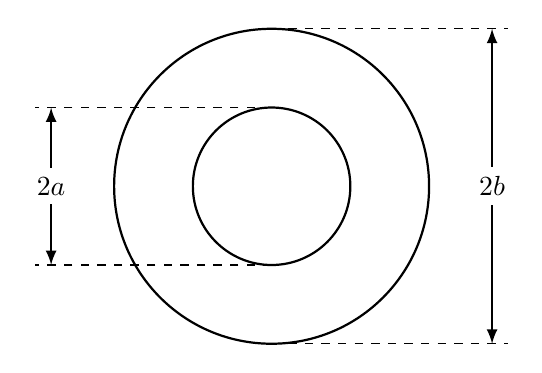
\begin{tikzpicture}
        %% outer loop
        \draw[thick] (0,0) circle (2);
        \draw[dashed] (0,+2) -- (3,+2);
        \draw[dashed] (0,-2) -- (3,-2);
        \draw[thick,latex-latex] (2.8,-2) -- (2.8,+2) node[pos=0.5,anchor=center,fill=white] {$2b$};
        %% inner loop
        \draw[thick] (0,0) circle (1);
        \draw[dashed] (0,+1) -- (-3,+1);
        \draw[dashed] (0,-1) -- (-3,-1);
        \draw[thick,latex-latex] (-2.8,-1) -- (-2.8,+1) node[pos=0.5,anchor=center,fill=white] {$2a$};
    \end{tikzpicture}
    \end{center}
    The larger loop carries an alternating current $I=I_0 \cos\omega t$,
        where $I_0$ and $\omega$ are constants.
    The magnetic field generated by the current in the large loop induces in the small loop an emf that is approximately equal to which of the following?
    (Either use mks units and let $\mu_0$ be the permeability of free space,
        or use Gaussian units and let $\mu_0$ be $4\pi / c^2$.)
    \begin{multicols}{2}
    \begin{choices}
        \wrongchoice{$\left(\dfrac{\pi\mu_0 I_0}{2}\right) \dfrac{a^2}{b}\omega \cos\omega t$}
        \wrongchoice{$\left(\dfrac{\pi\mu_0 I_0}{2}\right) \dfrac{a^2}{b}\omega \sin\omega t$}
        \wrongchoice{$\left(\dfrac{\pi\mu_0 I_0}{2}\right) \dfrac{a}{b^2}\omega \sin\omega t$}
        \wrongchoice{$\left(\dfrac{\pi\mu_0 I_0}{2}\right) \dfrac{a}{b^2} \cos\omega t$}
        \wrongchoice{$\left(\dfrac{\pi\mu_0 I_0}{2}\right) \dfrac{a}{b} \sin\omega t$}
    \end{choices}
    \end{multicols}
\end{question}
}

\element{gre}{
\begin{question}{GRE8677-Q82}
    The emission spectrum of an atomic gas in a magnetic field differs from that of the gas in the absence of a magnetic field.
    Which of the following is true of the phenomenon?
    \begin{choices}
        \wrongchoice{It is called the Stern-Gerlach effect.}
        \wrongchoice{It is called the Stark effect.}
        \wrongchoice{It is due primarily to the nuclear magnetic moment of the atoms.}
        \wrongchoice{The number of emission lines observed for the gas in a magnetic field is always twice the number observed in the absence of a magnetic field.}
        \wrongchoice{The number of emission lines observed for the gas in a magnetic field is either greater than or equal to the number observed in the absence of a magnetic field.}
    \end{choices}
\end{question}
}

\element{gre}{
\begin{question}{GRE8677-Q83}
    A spectral line is produced by a gas that is sufficiently dense that the mean time between atomic collisions is must shorter than the mean lives of the atomic states responsible for the line.
    Compared with the same line produced by a low-density gas,
        the line produced by the low-density gas,
        the line produced by the higher-density gas will appear
    \begin{choices}
        \wrongchoice{the same}
        \wrongchoice{more highly polarized}
        \wrongchoice{broader}
        \wrongchoice{shifted toward the blue end of the spectrum}
        \wrongchoice{split into a doublet}
    \end{choices}
\end{question}
}

\element{gre}{
\begin{question}{GRE8677-Q84}
    Sodium has eleven electrons and the sequence in which energy levels fill in atoms is $1s$, $2s$, $2p$, $3s$, $3p$, $4s$, $3d$, etc.
    What is the ground state of sodium in the usual notation $^{2S+1}L_j$?
    \begin{multicols}{3}
    \begin{choices}
        \wrongchoice{$^{1}S_0$}
        \wrongchoice{$^{2}S_{\frac{1}{2}}$}
        \wrongchoice{$^{1}P_{0}$}
        \wrongchoice{$^{2}P_{\frac{1}{2}}$}
        \wrongchoice{$^{3}P_{\frac{1}{2}}$}
    \end{choices}
    \end{multicols}
\end{question}
}

\element{gre}{
\begin{question}{GRE8677-Q85}
    \begin{center}
    \begin{tikzpicture}
        %% NOTE:
    \end{tikzpicture}
    \end{center}
    The figure above shows the photon interaction cross sections for lead in the energy range where the Compton, photoelectric, and pair production process all play a role.
    What is the correct identification of these cross section?
    \begin{choices}
        \wrongchoice{1=photoelectric, 2=Compton, 3=pair production}
        \wrongchoice{1=photoelectric, 2=pair production, 3=Compton}
        \wrongchoice{1=Compton, 2=pair production, 3=photoelectric}
        \wrongchoice{1=Compton, 2=photoelectric, 2=pair production}
        \wrongchoice{1=pair production, 2=photoelectric, 3=Compton}
    \end{choices}
\end{question}
}

\element{gre}{
\begin{question}{GRE8677-Q86}
    The exponent in Coulomb's inverse squared law has been found to differ from two by the less than one part in a billion by measuring which of the following?
    What is the correct identification of these cross section?
    \begin{choices}
        \wrongchoice{The charge on an oil drop in the Millikan experiment}
        \wrongchoice{The deflection of an electron beam in an electric field}
        \wrongchoice{The neutrality of charge of an atom}
        \wrongchoice{The electric force between two charged objects}
        \wrongchoice{The electric field inside a charged conducting shell}
    \end{choices}
\end{question}
}

\element{gre}{
\begin{question}{GRE8677-Q87}
    In a gas of $N$ diatomic molecules,
        two possible models for a classical description of a diatomic molecule are:
    \begin{center}
    \begin{tikzpicture}
        %% NOTE:
    \end{tikzpicture}
    \end{center}
    Which of the following statements about this gas is true?
    \begin{choices}
        \wrongchoice{Model I has a specific heat $c_v=\dfrac{3}{2}Nk$}
        \wrongchoice{Model II has a smaller specific heat than Model I}
        \wrongchoice{Model I is always correct}
        \wrongchoice{Model II is always correct}
        \wrongchoice{The choice between Models I and II depends on the temperature.}
    \end{choices}
\end{question}
}

\element{gre}{
\begin{question}{GRE8677-Q88}
    Consider a system of $N$ noninteracting particles confined in a volume $V$ at a temperature such that the particles obey classical Boltzmann statistics.
    If the temperature is lowered to the point at which quantum effects become important,
        the pressure of the gas may differ depending on whether the particles are fermions or bosons.
    Let $P_F$ be the pressure exerted by the particles if they are fermions,
        $P_B$ be the pressure if they are bosons,
        $P_C$ be the pressure the particles would exert if quantum effects are ignored.
    Which of the following is true?
    \begin{choices}
        \wrongchoice{$P_F = P_B = P_C$}
        \wrongchoice{$P_F > P_C > P_B$}
        \wrongchoice{$P_F > P_B > P_C$}
        \wrongchoice{$P_F < P_B < P_C$}
        \wrongchoice{$P_F < P_C < P_B$}
    \end{choices}
\end{question}
}

\element{gre}{
\begin{question}{GRE8677-Q89}
    A system containing two identical particles is described by a wave function of the form
    \begin{equation*}
        \Psi = \dfrac{1}{\sqrt{2}} \left[\Psi_{\alpha}(x_1) \Psi_{\beta}(x_2) + \Psi_{\beta}(x_1) \Psi_{\alpha}(x_2) \right]
    \end{equation*}
    where $x_1$ and $x_2$ represent the spatial coordinates of the particles $\alpha$ and $\beta$ represent all the quantum numbers,
        including spin, of the states that they occupy.
    The particle might be:
    \begin{multicols}{2}
    \begin{choices}
        \wrongchoice{electrons}
        \wrongchoice{positrons}
        \wrongchoice{protons}
        \wrongchoice{neutrons}
        \wrongchoice{deuterons}
    \end{choices}
    \end{multicols}
\end{question}
}

\element{gre}{
\begin{question}{GRE8677-Q90}
    \begin{center}
    \begin{tikzpicture}
        %% NOTE;
    \end{tikzpicture}
    \end{center}
    The figure above shows one of the possible energy eigenfunctions $\Psi(x)$ for a particle bouncing freely back and forth along the $x$-axis between impenetrable walls located at $x=-a$ and $x=+a$.
    The potential energy equals zero for $|x|<a$.
    If the energy  of the particle is 2 electron volts when it is in the quantum state associated with this eigenfunction,
        what is is energy when it is in the quantum state of lowest possible energy?
    \begin{multicols}{3}
    \begin{choices}
        \wrongchoice{$0\,\si{\eV}$}
        \wrongchoice{$\dfrac{1}{\sqrt{2}}\,\si{\eV}$}
        \wrongchoice{$\dfrac{1}{2}\,\si{\eV}$}
        \wrongchoice{$1\,\si{\eV}$}
        \wrongchoice{$2\,\si{\eV}$}
    \end{choices}
    \end{multicols}
\end{question}
}

\element{gre}{
\begin{question}{GRE8677-Q91}
    What a narrow beam of monochromatic electrons impinges on the surface of a single metal crystal at an angle of 30 degrees with the plane of the surface,
        first-order reflection is observed.
    If the spacing of the reflecting crystal planes is known from x-ray measurements to be 3 \r{a}ngstroms,
        the speed of the electrons is most nearly:
    \begin{multicols}{2}
    \begin{choices}
        \wrongchoice{\SI{1.4e-4}{\meter\per\second}}
        \wrongchoice{\SI{2.4}{\meter\per\second}}
        \wrongchoice{\SI{5.0e8}{\meter\per\second}}
        \wrongchoice{\SI{2.4e6}{\meter\per\second}}
        \wrongchoice{\SI{4.5e9}{\meter\per\second}}
    \end{choices}
    \end{multicols}
\end{question}
}

\element{gre}{
\begin{question}{GRE8677-Q92}
    Which of the following is \emph{not} compatible with the selection rule that controls electric dipole emission of photons by excited states of atoms?
    \begin{choices}
        \wrongchoice{$\Delta n$ may have any negative integral value.}
        \wrongchoice{$\Delta l = \pm 1$}
        \wrongchoice{$\Delta m_l = 0, \pm 1$}
        \wrongchoice{$\Delta s = \pm 1$}
        \wrongchoice{$\Delta j = \pm 1$}
    \end{choices}
\end{question}
}

\element{gre}{
\begin{question}{GRE8677-Q93}
    \begin{center}
    \begin{tikzpicture}
        %% NOTE:
    \end{tikzpicture}
    \end{center}
    An electric sander has a continuous belt that rubs against a wood surface as shown schematically above.
    The sander is 100 percent efficient and draws a current of 9 amperes from a 120 volt line.
    The belt speed is 10 meters per second.
    If the sander is pushing against the wood with a normal force of 100 newtons,
        the coefficient of friction is most nearly:
    \begin{multicols}{3}
    \begin{choices}
        \wrongchoice{0.02}
        \wrongchoice{0.2}
        \wrongchoice{0.4}
        \wrongchoice{1.1}
        \wrongchoice{10}
    \end{choices}
    \end{multicols}
\end{question}
}

\element{gre}{
\begin{question}{GRE8677-Q94}
    \begin{center}
    \begin{tikzpicture}
        %% NOTE:
    \end{tikzpicture}
    \end{center}
    In the circuit shown above, $R_2=3R_1$ and the battery of emf $\xi$ has negligible integral resistance.
    The resistance of the diode when it allows current to pass through it is also negligible.
    At time $t=0$,
        the switch $S$ is closed and the currents and voltages are allowed to reach their asymptotic values.
        Then at time $t_1$, the switch is opened.
    Which of the following curves most nearly represents the potential at point $A$ as a function of time $t$?
    \begin{multicols}{2}
    \begin{choices}
        \wrongchoice{
            \begin{tikzpicture}
                %% NOTE: TODO: pgfplots
            \end{tikzpicture}
        }
    \end{choices}
    \end{multicols}
\end{question}
}

\element{gre}{
\begin{question}{GRE8677-Q95}
    \begin{center}
    \begin{tikzpicture}
        %% NOTE:
    \end{tikzpicture}
    \end{center}
    In the cycle shown above, $KL$ and $NM$ represent isotherms, while $KN$ and $LM$ represent reversible adiabats.
    A system is carried through the Carnot cycle $KLMN$, taking in heat $Q_2$ from the hot reservoir $T_2$ and releasing heat $Q_1$ to the cold reservoir $T_1$.
    All of the following statements are true \emph{except}:
    \begin{choices}
        \wrongchoice{$Q_1/T_1 -= Q_2/T_2$}
        \wrongchoice{The entropy of the hot reservoir decreases.}
        \wrongchoice{The entropy of the system increases.}
        \wrongchoice{The work $W$ done is equal to the net heat absorbed, $Q_2 - Q_1$}
        \wrongchoice{The efficiency of the cycle is independent of the working substance.}
    \end{choices}
\end{question}
}

\element{gre}{
\begin{question}{GRE8677-Q96}
    A particle of mass $M$ is in an infinitely deep square well potential $V$ where
    \begin{equation*}
        %% NOTE: TODO: table for statments
    \end{equation*}
    A very small perturbing potential $V\prime$ is superimposed on $V$ such that
    \begin{equation*}
        %% NOTE: TODO: table for statments
    \end{equation*}
    \begin{choices}[o]
        \wrongchoice{$\Psi_0^{\prime} = a_{00} \Psi_0, a_{00} \neq 0$}
        \wrongchoice{$\Psi_0^{\prime} = \sum_{n=0}^{\infty} a_{0n} \Psi_n$ with $a_{0n}=0$ for all odd values of $n$}
        \wrongchoice{$\Psi_0^{\prime} = \sum_{n=0}^{\infty} a_{0n} \Psi_n$ with $a_{0n}=0$ for all even values of $n$}
        \wrongchoice{$\Psi_0^{\prime} = \sum_{n=0}^{\infty} a_{0n} \Psi_n$ with $a_{0n}\neq 0$ for all values of $n$}
        \wrongchoice{None of the above}
    \end{choices}
\end{question}
}

\element{gre}{
\begin{question}{GRE8677-Q97}
    \begin{center}
    \begin{tikzpicture}
        %% NOTE:
    \end{tikzpicture}
    \end{center}
    Two uniform cylindrical disks of identical mass $M$, radius $R$, and moment of inertia $\frac{1}{2}MR^2$, as shown above, collide on a frictionless, horizontal surface.
    Disk I, having an initial counterclockwise angular velocity $\omega_0$ and a center-of-mass velocity $v_0 = \frac{1}{2}\omega_0 R$ to the right,
        makes a grazing collision with disk II initially at rest.
    If after the collision the two disks stick together,
        the magnitude of the total angular momentum about the point $P$ is:
    \begin{multicols}{2}
    \begin{choices}
        \wrongchoice{zero}
        \wrongchoice{$\dfrac{1}{2} M R^2 \omega_0$}
        \wrongchoice{$\dfrac{1}{2} M R v_0$}
        \wrongchoice{$M R v_0$}
        \wrongchoice{dependent on the time of the collision}
    \end{choices}
    \end{multicols}
\end{question}
}

\element{gre}{
\begin{question}{GRE8677-Q98}
    \begin{center}
    \begin{tikzpicture}
        %% NOTE:
    \end{tikzpicture}
    \end{center}
    The long thin cylindrical glass rod shown above has length $l$ and is insulated from its surroundings.
    The rod has an excess charge $Q$ uniformly distributed along its length.
    Assume the electric potential to be zero at infinite distance from the rod.
    If $k$ is the constant in Coulomb's law,
        the electric potential at a point $P$ along the axis of the rod and a distance $l$ from one end is $\frac{kQ}{l}$ multiplied by:
    \begin{multicols}{3}
    \begin{choices}
        \wrongchoice{$\dfrac{4}{9}$}
        \wrongchoice{$\dfrac{1}{2}$}
        \wrongchoice{$\dfrac{2}{3}$}
        \wrongchoice{$\ln 2$}
        \wrongchoice{$1$}
    \end{choices}
    \end{multicols}
\end{question}
}

\element{gre}{
\begin{question}{GRE8677-Q99}
    The positronium ``atom'' consists of an electron and a positron bound together by their mutual Coulomb attraction and moving about their center of mass,
        which is located halfway between them.
    Thus the positronium ``atom'' is somewhat analogous to a hydrogen atom.
    The ground-state binding energy of hydrogen is 13.6 electron volts.
    What is the ground-state binding energy of positronium?
    \begin{multicols}{2}
    \begin{choices}
        \wrongchoice{$\left(\dfrac{1}{2}\right)^2 \times \SI{13.6}{\eV}$}
        \wrongchoice{$\dfrac{1}{2} \times \SI{13.6}{\eV}$}
        \wrongchoice{$\SI{13.6}{\eV}$}
        \wrongchoice{$2 \times \SI{13.6}{\eV}$}
        \wrongchoice{$\left(2\right)^2 \times \SI{13.6}{\eV}$}
    \end{choices}
    \end{multicols}
\end{question}
}

\element{gre}{
\begin{question}{GRE8677-Q100}
    The screen of a pinhole camera is at a distance $D$ from the pinhole,
        which has a diameter $d$.
    The light has an effective wavelength $\lambda$, $\left(\lambda \ll D\right)$.
    For which of the  following values of $d$ will the image be sharpest?
    \begin{multicols}{3}
    \begin{choices}
        \wrongchoice{$\sqrt{\lambda D}$}
        \wrongchoice{$\lambda$}
        \wrongchoice{$\dfrac{\lambda}{10}$}
        \wrongchoice{$\dfrac{\lambda^2}{D}$}
        \wrongchoice{$\dfrac{D^2}{\lambda}$}
    \end{choices}
    \end{multicols}
\end{question}
}


\endinput

